\documentclass[a5paper]{article}

\usepackage[english,russian]{babel} % russian typesetting standards
\usepackage[T2A]{fontenc} % so that we could use cyrillic sybols at all
\usepackage[warn]{mathtext} % use cyrillic symbols in formulas
\usepackage{babelbib}
\usepackage{amsfonts, amsmath, amssymb, amsthm} % AMS math typesetting & fonts
\usepackage[margin=.7in]{geometry} % just margins
\usepackage{tikz} % fancy pictures
\usepackage{framed} % frames for important things
\usepackage{hyperref}
\hypersetup{
    colorlinks,
    citecolor=black,
    filecolor=black,
    linkcolor=black,
    urlcolor=black
}

\newtheorem{definition}{Определение}
\newtheorem{theorem}{Теорема}
\newtheorem{lemma}{Лемма}
\newtheorem{statement}{Утверждение}
\newtheorem{remark}{Замечание}
\newtheorem{exercise}{Упражнение}
\newtheorem{corollary}{Следствие}
\newtheorem{example}{Пример}

\DeclareMathOperator*\res{res}
\DeclareMathOperator\im{Im}
\DeclareMathOperator\re{Re}
\DeclareMathOperator\supp{supp}


\author{Павел Иевлев}
\title{Metapost}
\date{}

\begin{document}

\maketitle

\begin{figure}[h]
  \centering
  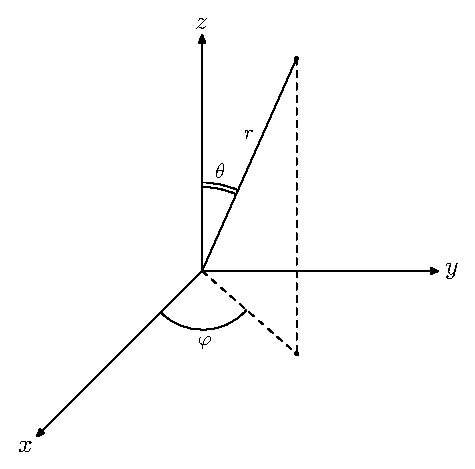
\includegraphics{spherical_coordinates.eps}
  \caption{spherical coordinates}
  \label{fig:spherical_coordinates}
\end{figure}

\begin{figure}[h]
  \centering
  
\includegraphics{moebius-35deg.eps}
  \caption{moebius strip, 35 deg}
  \label{fig:moebius-35deg}
\end{figure}

\begin{figure}[h]
  \centering
  
\includegraphics{moebius-65deg.eps}
  \caption{moebius strip, 65 deg}
  \label{fig:moebius-65deg}
\end{figure}

\end{document}
